\section{Simulation Results}
\label{sec:simulation}
\Matt{BLUE: I would not mind removing this text. RED: I will likely remove this text}
The simulation results are consistent across all the PARSEC benchmarks. The reason for this consistency is due to the similarity of the memory traces across the benchmarks. Given sufficient memory overhead, we see that we consistently achieve a roughly 25\% improvement over the baseline simulation. We find that the Coding Scheme I generally performs the best out of the proposed schemes. 

\subsection{PARSEC Results}

The proposed memory system performs consistently across the PARSEC benchmarks, and the three proposed schemes yield similar results. Figure~\ref{fig:dedup_results} shows the simulation results for the dedup benchmark. The plot shows that the number of CPU cycles is reduced by between 83\% and 73\% once a sufficient amount of memory is provided to the memory system. The lines on this figure and others show the number of CPU cycles needed for the Ramulator simulation to finish executing. The bars on these graphs show the number of times the dynamic encoder chooses to encode a new memory region due to the number of memory requests coming from that region. We note that when $\alpha = 1$, the number of switches is always zero because the dynamic encoder never needs to switch regions.

These results were simulated using a memory partition coefficient $r = .05$. We observe that the performance remains consistent for $\alpha > .1$. The reason for this is that there are two heavily accessed memory bands in each of the PARSEC benchmarks. Once the memory system is able to encode both of these regions, the benefits of the memory system are fully realized. At an $\alpha = .1$, the memory system finds and encodes the two heavily accessed memory bands. $\alpha = .1$ is sufficient to encode the two heavily accessed memory bands because $\lfloor\frac{\alpha}{r}\rfloor = 2$, so the memory system can select 2 regions to encode. The number of coded region switches is evidence that at $\alpha = .05$ more memory is needed to see maximum benefits from the memory system. When $\alpha = .05$, the number of switches is very high because the memory system vacillates between the two most heavily accessed bands. When $\alpha = .1$, the number of switches is nearly zero because the memory system can only select two memory regions to encode, and it seldom has a reason to switch away from the two heavily accessed bands. We see small numbers of switches when $\alpha = {.2, .25, .5}$ because the memory system is encoding less heavily accesses memory bands.

\begin{figure}[htbp]
		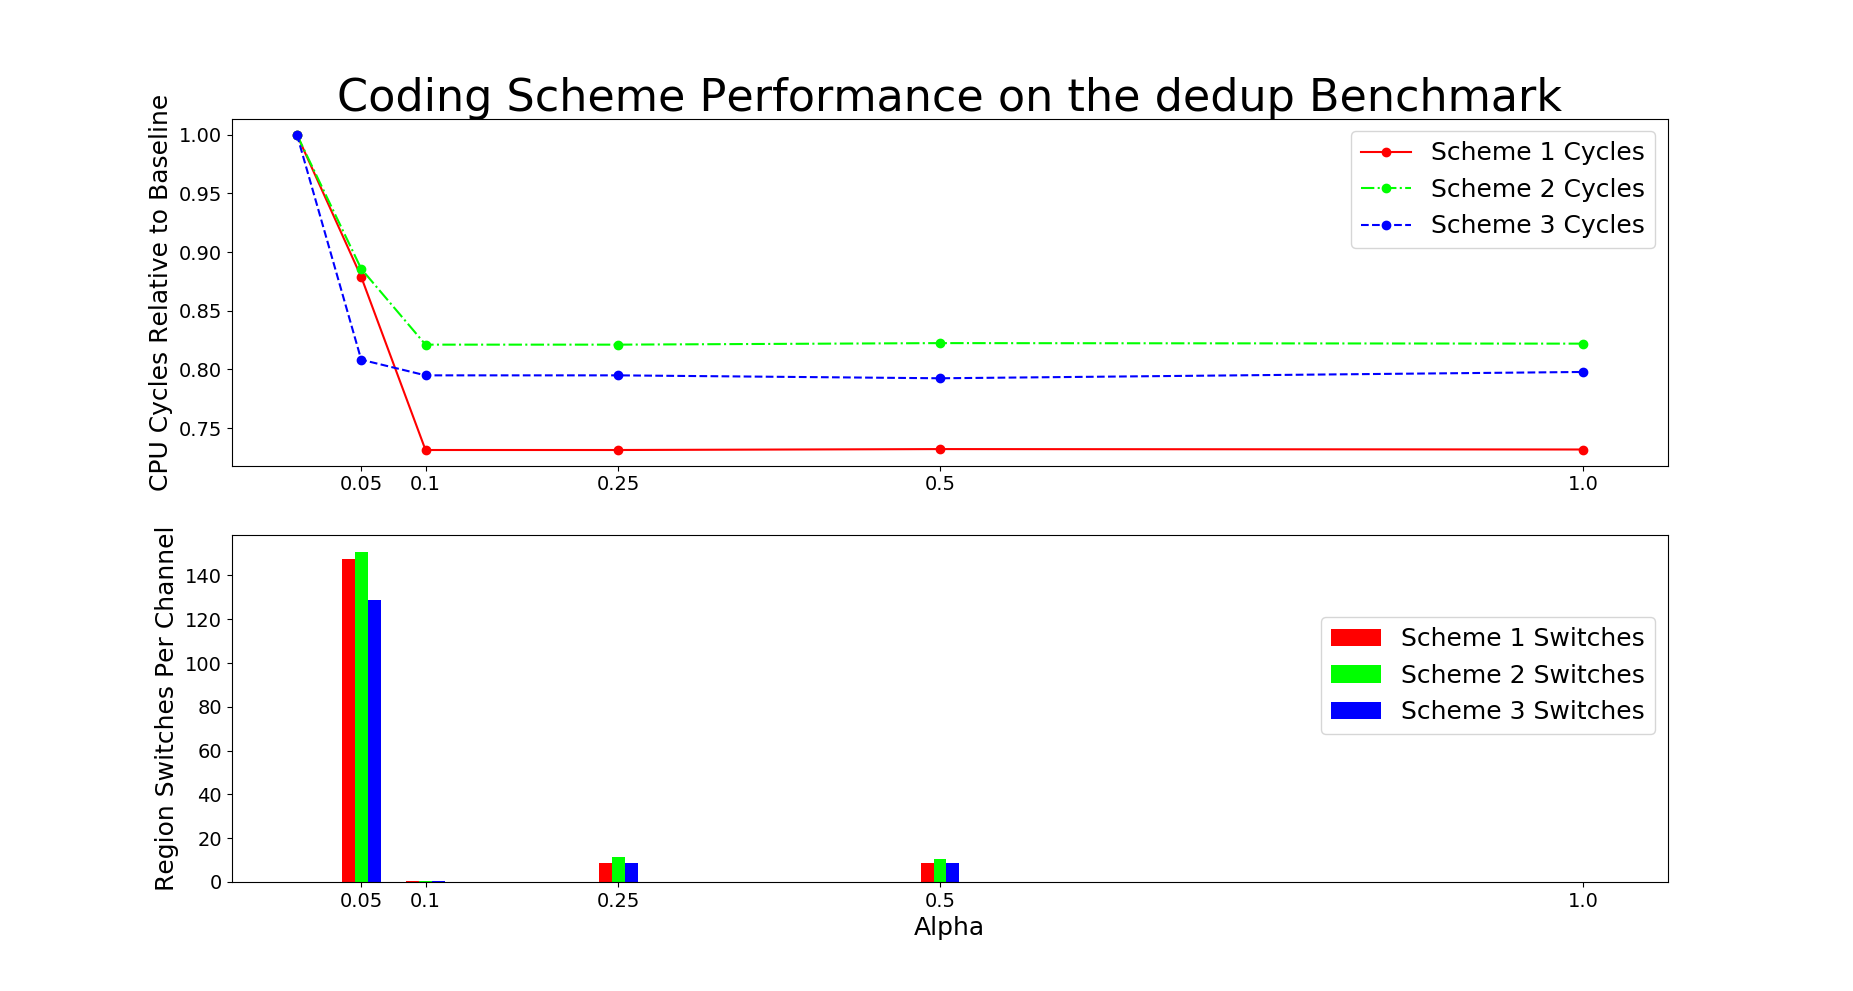
\includegraphics[width=\linewidth]{fig/dedup_benchmark_results.png}
		\caption{The simulation results for the dedup PARSEC benchmark. The line plot represents the number of CPU cycles needed and the bar plot represents the number of tiems the dynamic coding unit chooses to encode a new memory region. The results from the other PARSEC benchmarks are very similar to those seen here.}
		\label{fig:dedup_results}
\end{figure}

\begin{figure}[htbp]
		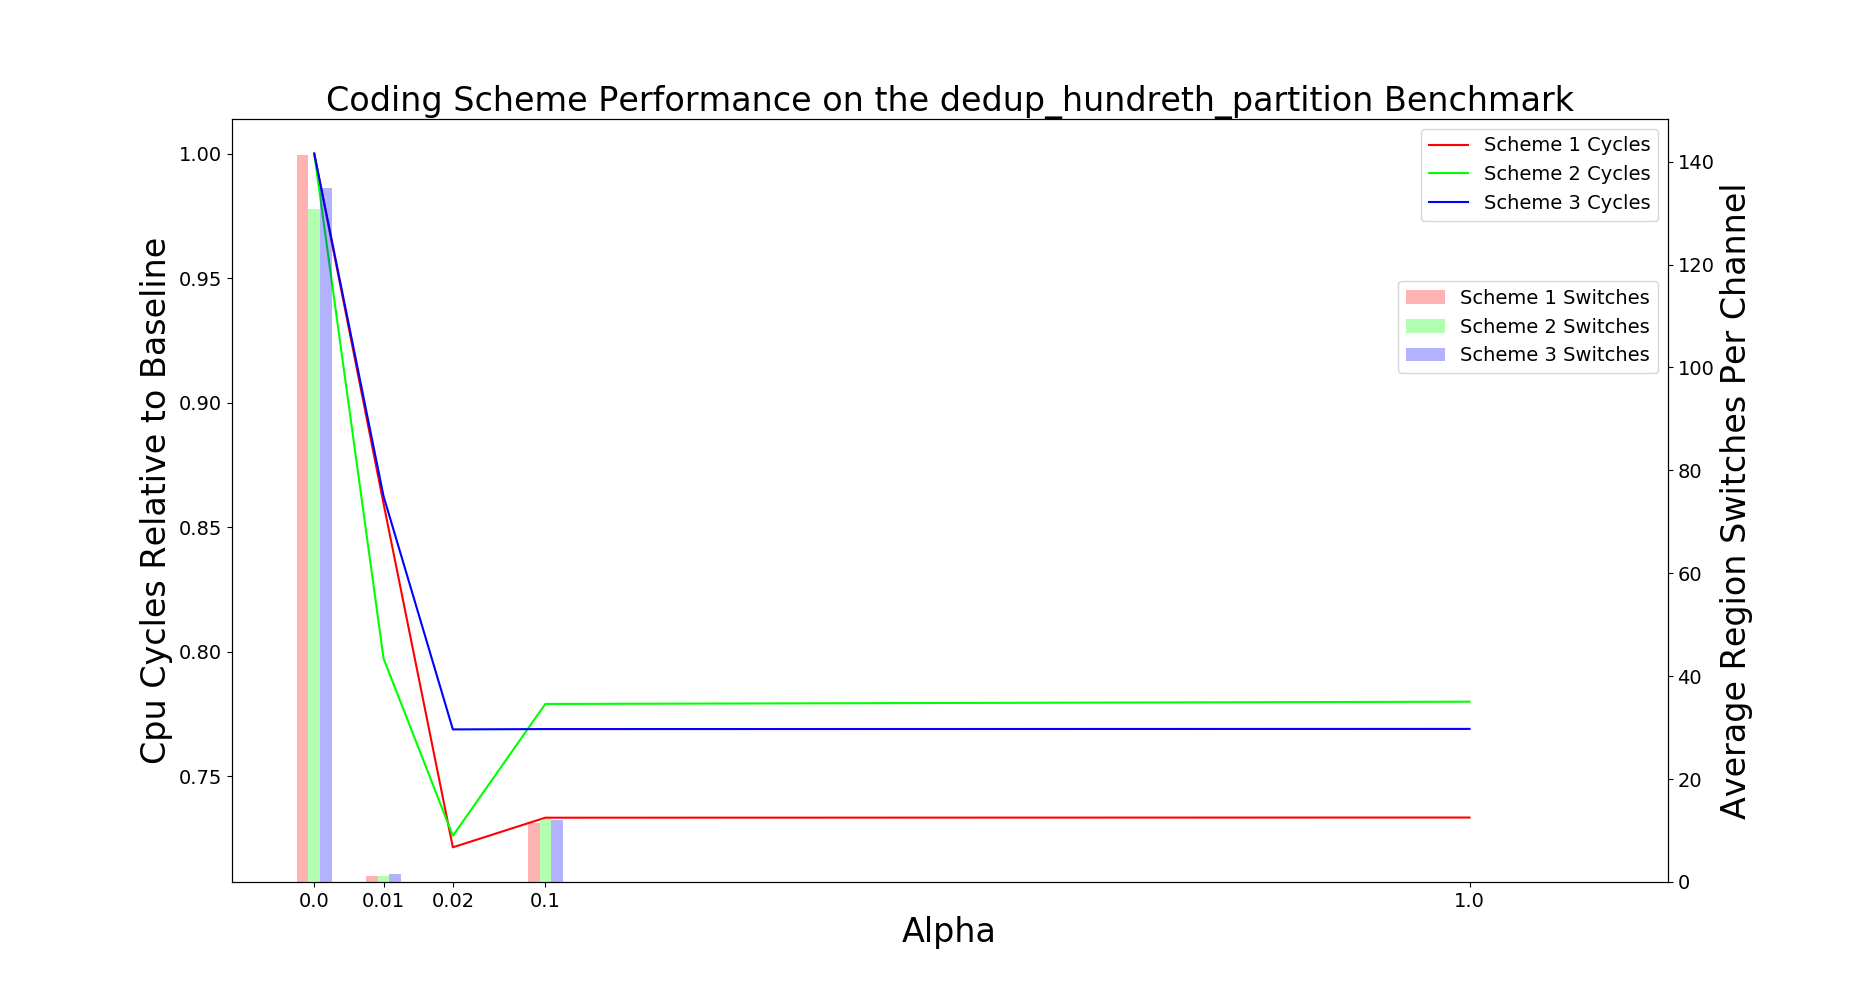
\includegraphics[width=\linewidth]{fig/dedup_hundreth.png}
		\caption{The simulation results for the same trace simulated in Figure~\ref{fig:dedup_results} but with a memory partition coefficient $r = .01$}
		\label{fig:dedup_hundreth}
\end{figure}

The heavily accesses memory bands are narrow, so decreasing the memory bank partition to allows us to lower $\alpha$ and see no decrease in performance. This is demonstrated by Figure~\ref{fig:dedup_hundreth}. Here, it is shown that we can reduce 5 times more than the previous simulation. This is achieved by decreasing the memory partition coefficient $r$ from .05 to .01.


\subsection{PARSEC Augmentation}
Because the PARSEC benchmarks are homogenous in structure, we chose to augment them in order to observe how the proposed memory system performs in more scenarios. The PARSEC benchmarks were augmented in two ways. The first augmentation is to split the memory bands observed in Figure~\ref{fig:dedup_whole} and Figure~\ref{fig:dedup_dense} into a greater number of bands. The second augmentation was to ramp the memory bands over time. A visualization of the augmented traces can be seen in Figure~\ref{fig:vips_split} and~\ref{fig:vips_ramp}

\begin{figure}[htbp]
		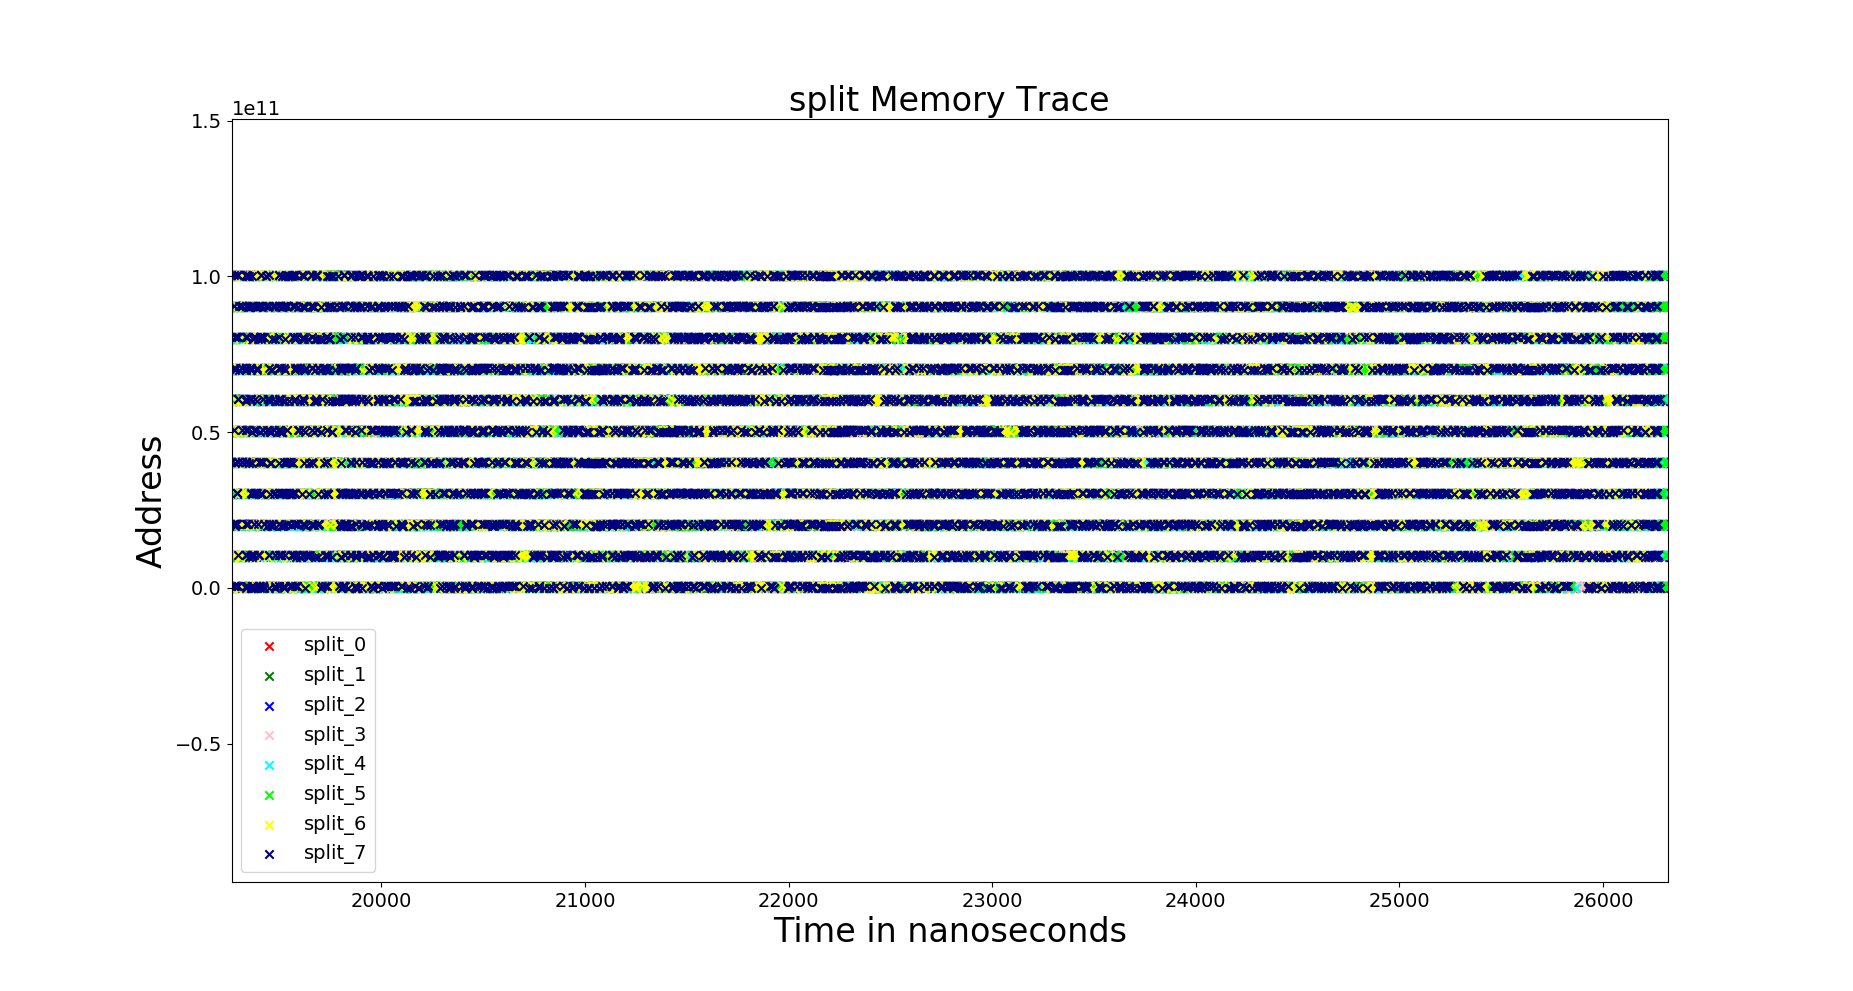
\includegraphics[width=\linewidth]{fig/vips_split.png}
		\caption{The vips benchmark after the major memory access bands were split into a greater number of bands}
		\label{fig:vips_split}
\end{figure}


\begin{figure}[htbp]
		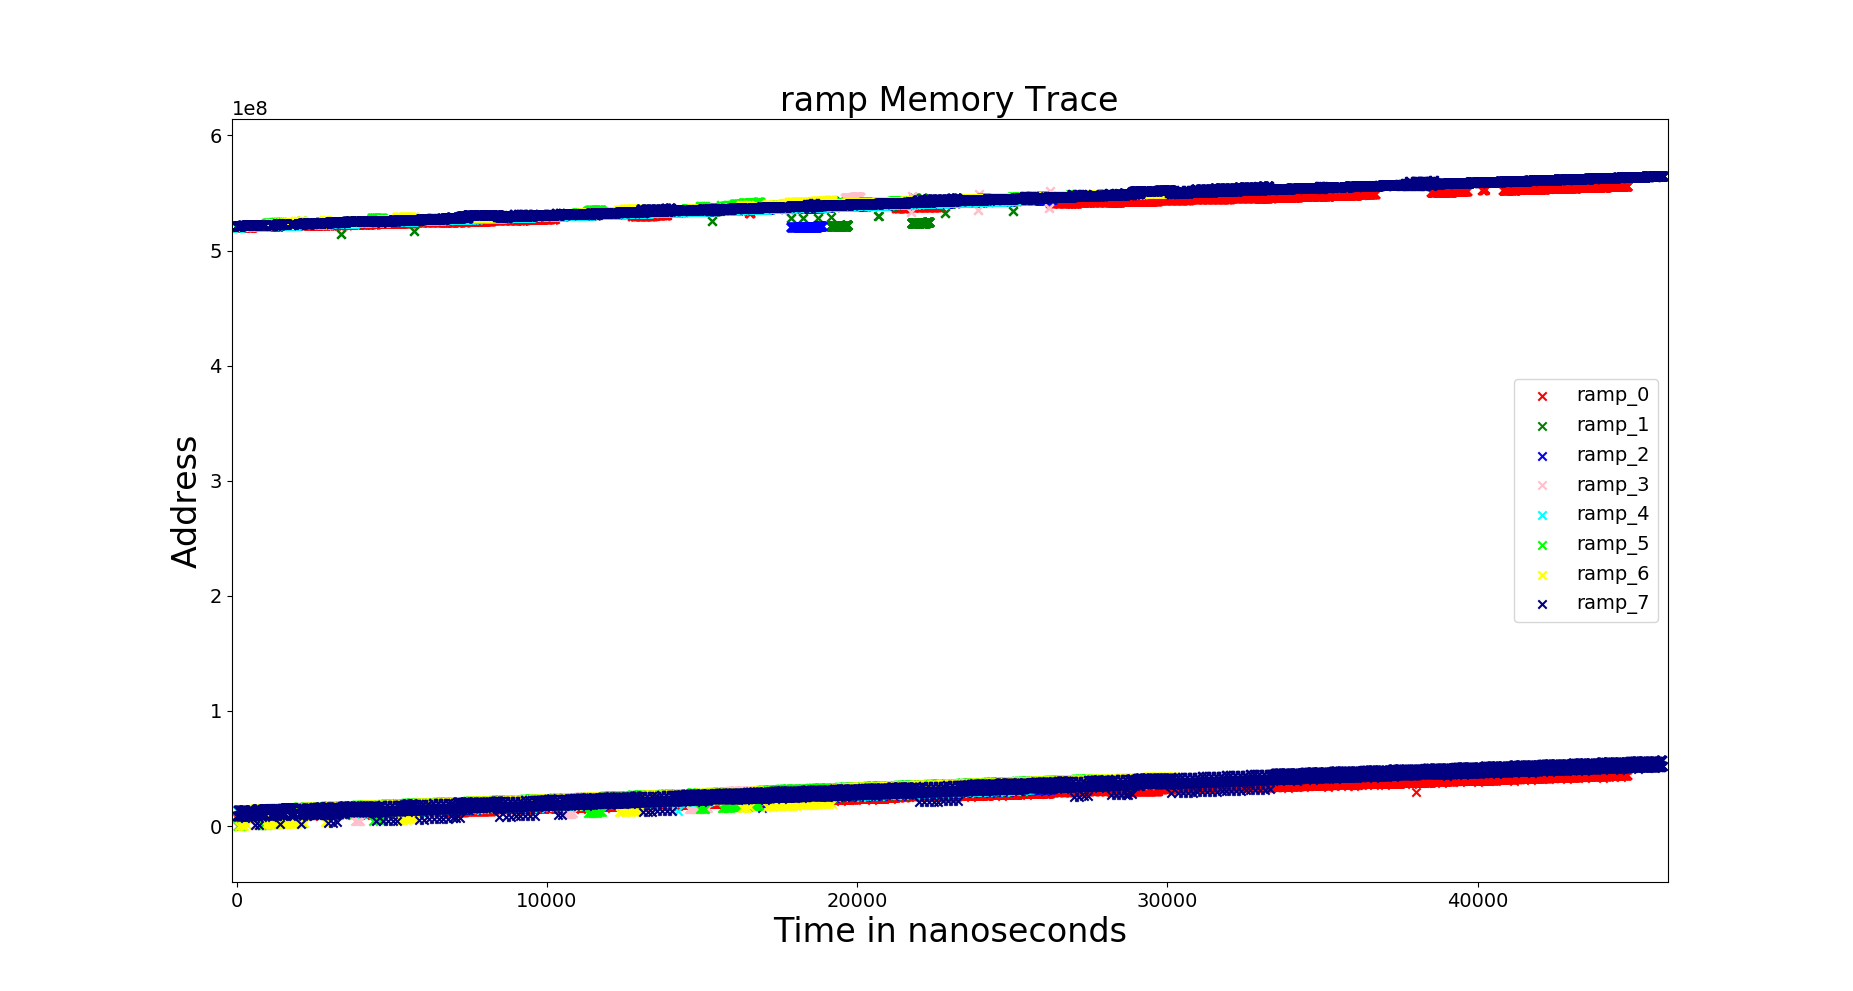
\includegraphics[width=\linewidth]{fig/vips_ramp.png}
		\caption{The vips benchmark after a ramp was added to the major memory bands}
		\label{fig:vips_ramp}
\end{figure}

\subsection{Augmented PARSEC Results}

The augmented PARSEC results significantly impact the Ramulator simulation results. Increasing the number of memory bands by splitting the dense bands results in an increased memory requirement to see improved performance. Introducing a ramp to the memory bands decreases the efficacy of the proposed memory system across all values of $\alpha$.

Figure~\ref{fig:vips_split_result} shows the results from the split augmentation. When there are large number of memory bands, the proposed memory system can achieve the same performance as when there are fewer memory bands if the memory overhead of the system is increased. Note that the simulation results in Figure~\ref{fig:vips_split_result} can be achieved using less memory by decreasing the memory partition coefficient. The memory partition coefficient used here is $r = .05$, but as shown in Figures ~\ref{fig:dedup_results} and ~\ref{fig:dedup_hundreth} lowering the memory partition coefficient allows a lowering of $\alpha$ while achieving the same performance.

Figure~\ref{fig:vips_ramp_result} shows the results of the ramp augmentation. The proposed memory system performace worse in this scenario. The number of memory region switches shows that the memory system struggles to handle the constantly changing location of the heavily accessed memory regions. In the other simulator results, we see that the number of memory region switches decreases as a function of $\alpha$. The reason for this is that the memory system locates the heavily accessed memory regions and rarely switches away from them. Here, the memory system is constantly attempting to catch up with the heavily accessed memory region. {\color{blue}We note that the ramp covers a very large number of memory addresses, so the decrease in performance we observe would only effect programs which use very large portions of memory.} 

\begin{figure}[htbp]
		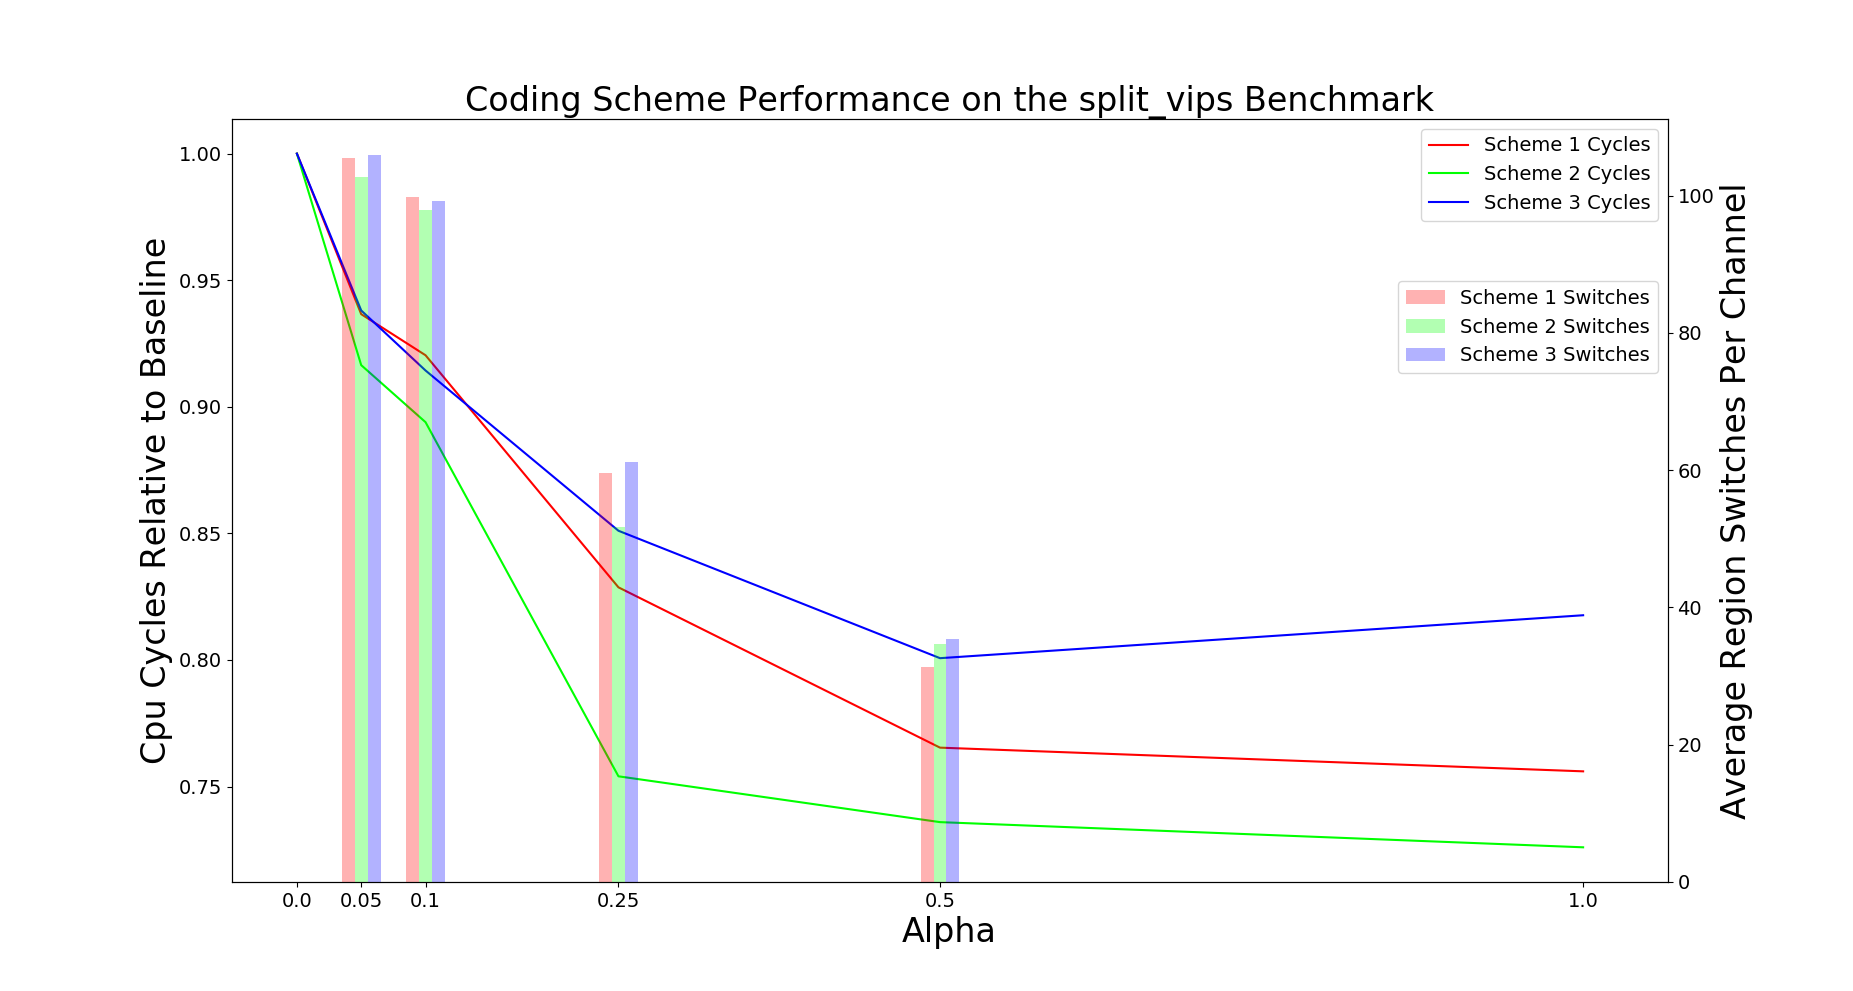
\includegraphics[width=\linewidth]{fig/vips_split_results.png}
		\caption{The simulation results of the augmented vips trace pictured in Figure~\ref{fig:vips_split}}
		\label{fig:vips_split_result}
\end{figure}

\begin{figure}[htbp]
		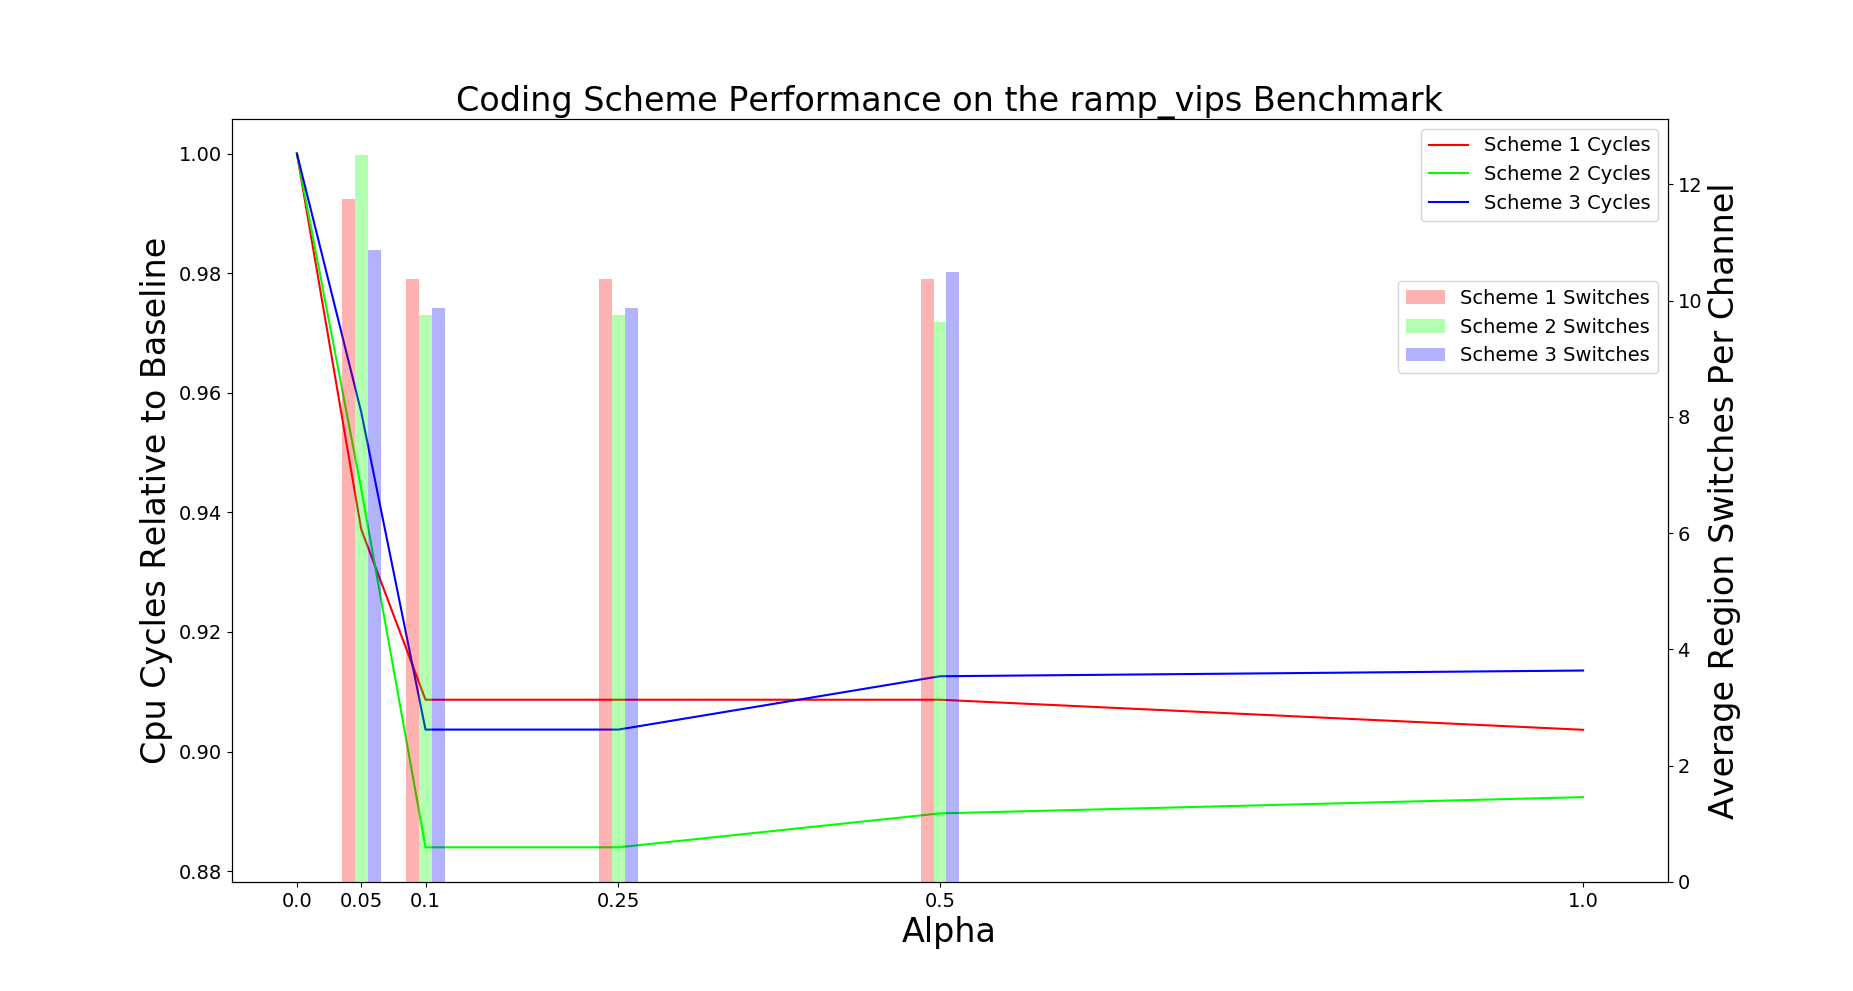
\includegraphics[width=\linewidth]{fig/vips_ramp_results.png}
		\caption{The simulation results of the augmented vips trace pictured in Figure~\ref{fig:vips_ramp}}
		\label{fig:vips_ramp_result}
\end{figure}


